\chapter{Introduction}
This chapter discusses key points about this final project, i.e. motivation, problem formulation, limitation of study, objective of study, and systematic writing.

\section{Motivation}
Emergency is an abnormal event that has negative impact because it can threaten and disrupt a person's life. Emergency occurs suddenly with unexpected place and time. An emergency can be presented in many forms; from everyday incidents like traffic accident or assault, to major incidents like wildfire, earthquake, or large-scale terrorist attacks.

Many fatal impact in emergency situation can be prevented or reduced by adequate first aid. Therefore, most countries have implemented some form of emergency services in order to do first aid in emergency. In Indonesia, emergency services divided into several hotline which are 118 for ambulance services, 110 for police services, and 113 for fire brigade services. On December 2016, KOMINFO implementing single hotline number 112 emergency services as an experiment project for some cities. One of those cities is Bandung.

The 112 emergency services  aims to establish an easy recall number that can be accessed by anyone, anytime, anywhere. It provides services of ambulance, police, and fire brigade. This emergency service works as a bridge connecting user to each emergency units. On June 2017,  112 emergency services in Bandung received 637 emergency requests. It means over 21 emergency requests received per day by specially trained operators. The operator have to decide which nearest emergency unit to dispatch to emergency location every time emergency happens. The environment they operate is characterized by high degree of uncertainty. Its because they don't know the exact distance from each unit to emergency location which inconvenience them to determining nearest emergency unit.

\pagebreak

\begin{figure}[H]
    \centering
    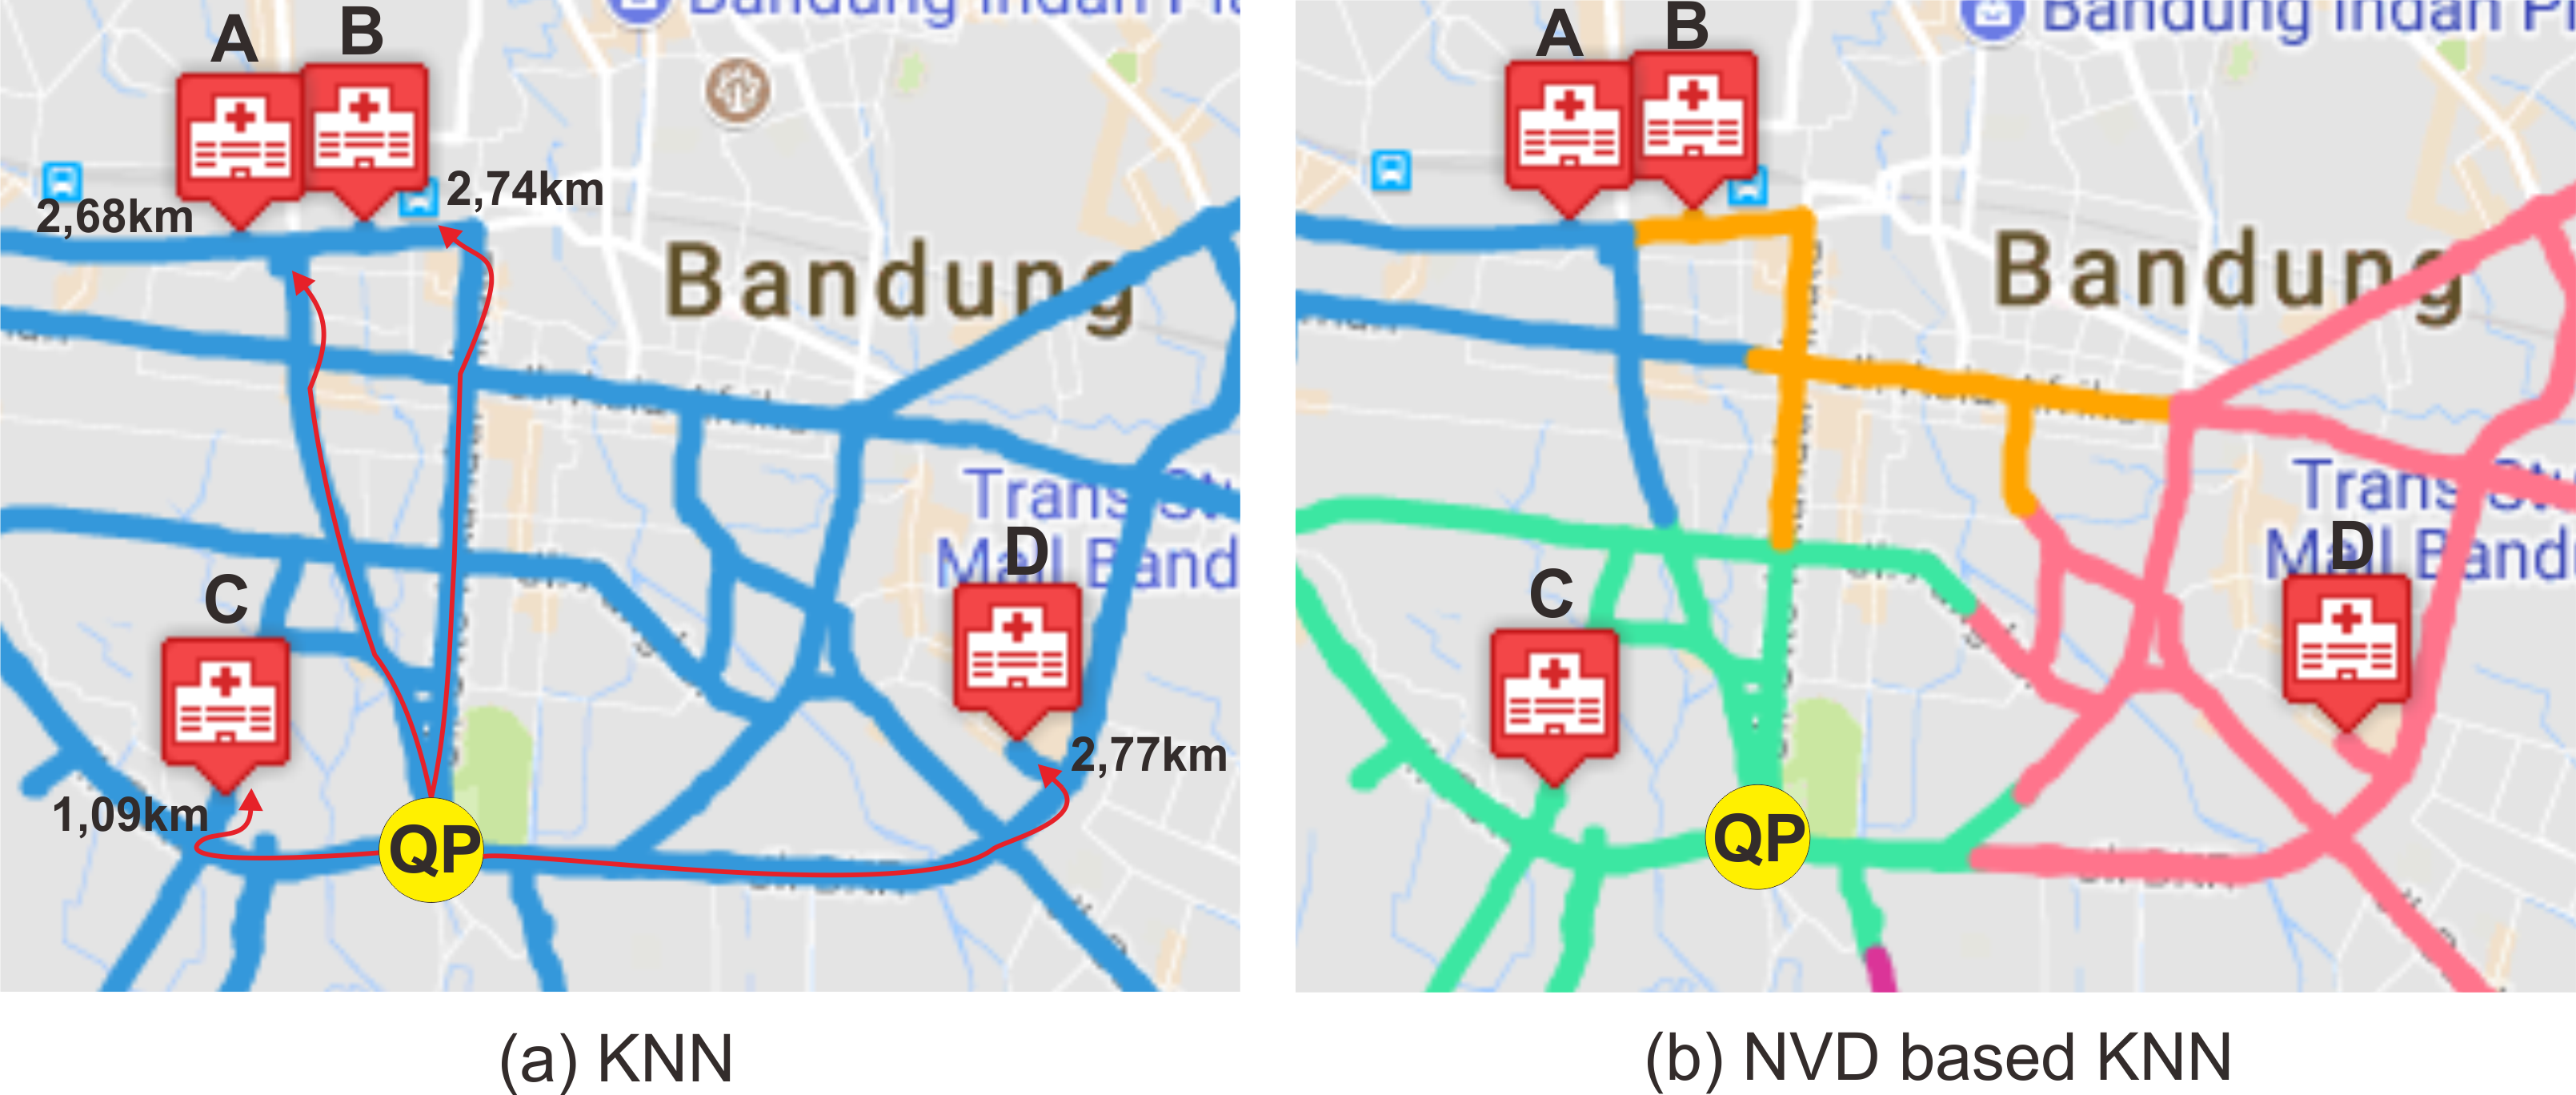
\includegraphics[scale=0.5]{illustration.png}
    \caption{Emergency services illustration in Bandung}
    \label{fig:illustration}
\end{figure}

In computer science, finding nearest emergency unit can be determine by using K-Nearest Neighbor (KNN) algorithm. Consider road network in Bandung shown in figure \ref{fig:illustration}(a), where emergency happens in Query Point (QP). KNN needs to determine each emergency unit distance to QP before comparing it and pick up the emergency unit with minimum distance. So in figure \ref{fig:illustration}(a), the nearest ambulance is C-ambulance. Notice that if there are emergency requests from many different location, then these process will repetead for each request. More requests means more processes KNN will takes.

Each emergency unit basically has a coverage area which specifies that its closer to the emergency unit than others. It can be done by using Network Voronoi Diagram (NVD) algorithm. NVD works as shown in figure \ref{fig:illustration}(b), where every road network's color represented each emergency unit's territories. So when emergency happens, NVD just needs to determine which emergency unit's territory emergency exist. In figure \ref{fig:illustration}(b) QP exist in C-ambulance with green territory which is the nearest ambulance.

This final project presents Network Voronoi Diagram based K-Nearest Neighbor development for 3 emergency services (ambulance, police, and fire brigade) in Bandung. In general, when an emergency occurs, user contact 112 to make a report. System will determine user coordinate location and select nearest emergency unit. System also support finding next nearest emergency units if nearest unit is on duty. The selected unit will be dispatch after receiving shortest path to the emergency location.

\pagebreak

\section{Problem Formulation}
Based on facts and problems mentioned in subsection motivation above, the main problems which will be discussed in this final project as follows :
\begin{enumerate}
	\item How to get k-nearest emergency unit to emergency location?
    \item How to find shortest path from selected units to emergency location?
\end{enumerate}

\section{Limitation of the Study}
To scope this final project to be more specific in accordance with the title and purpose, this final project limited to be discussed as follows :
\begin{enumerate}
    \item This final project only focused on emergency services in Bandung but only in west, south, east region.
    \item The road network used is the road segments that have functions as primary arterial roads, primary collector roads, secondary arterial road, and secondary collector road.
    \item Emergency units are divided into ambulance, police and fire brigade.
    \item Emergency unit selected is based on k-nearest from emergency location.
    \item Route determination from selected units to emergency location using shortest path ignoring road conditions.
\end{enumerate}


\section{Objective of the Study}
Based on the formulation of the above problems, this final project's objective are described as follows:
\begin{enumerate}
    \item To help operators determining k-nearest emergency unit from emergency location.
    \item To generate shortest path from emergency unit to emergency location so these unit can do first aid before fatal injury happens.
\end{enumerate}


\pagebreak
\iflogTA
\section{Systematic Writing}
The writing of the results in this report follows the description given in each successive chapter to facilitate discussion. From the subject matter can be divided into six chapters as described below :
\begin{enumerate}[label=Chapter I \hspace{5mm} : \hspace{2mm}, leftmargin=*, topsep=0pt, itemsep=-1ex, partopsep=1ex, parsep=1ex]
\item Introduction chapter contains an introduction that includes background, problem formulation, limitation of the study, objective of study, and systematic writing.
\end{enumerate}
\begin{enumerate}[label=Chapter II \hspace{3.5mm} : \hspace{2mm}, leftmargin=*, topsep=0pt, itemsep=-1ex, partopsep=1ex, parsep=1ex]
\item Review of Related Literature\\This chapter contains the theoretical foundations that support and directly relate to research to be conducted from books, research journals, internet, and other literary sources.
\end{enumerate}
\begin{enumerate}[label=Chapter III \hspace{2mm} : \hspace{2mm}, leftmargin=*, topsep=0pt, itemsep=-1ex, partopsep=1ex, parsep=1ex]
\item Method of Investigation\\This chapter contains a description of the steps of research conducted, but it is also a picture of author's mind frame in doing this final project from the beginning until it completed.
\end{enumerate}
\begin{enumerate}[label=Chapter IV \hspace{2mm} : \hspace{2mm}, leftmargin=*, topsep=0pt, itemsep=-1ex, partopsep=1ex, parsep=1ex]
\item Data Collection and Processing \\This chapter contains data collection process used in tis final project and contains process of data processing as an effort to create solutions for existing problems.
\end{enumerate}
\begin{enumerate}[label=Chapter V \hspace{3.5mm} : \hspace{2mm}, leftmargin=*, topsep=0pt, itemsep=-1ex, partopsep=1ex, parsep=1ex]
\item Result Analysis\\This chapter contains the analysis and data interpretation of the results in the previous section. The purpose of this section is to provide clear information about the results of this final project and able to provide solutions of the problems that arise.
\end{enumerate}
\begin{enumerate}[label=Chapter VI \hspace{2mm} : \hspace{2mm}, leftmargin=*, topsep=0pt, itemsep=-1ex, partopsep=1ex, parsep=1ex]
\item Conclusion\\This chapter contains the conclusions derived from the system design and analysis that have been done and the recommendations given for improvement.
\end{enumerate}
\else
\section{Plan Activity}
\begin{itemize}
	\item Study of literature
	
	At this stage, author tries to learn the concepts and theories about Network Voronoi Diagram also K-Nearest Neighbor from existing literature in books or international papers.
	\item Collecting Data

At this stage, author collecting necessary data as dataset by searching for information in advance on the internet and confirm it to speaker who are more competent.
\pagebreak
	\item Design and Implementation System

At this stage, author designing and implementation Network Voronoi Diagram KNN for building the system from problems.
	\item Testing and Analysis Results

In this stage, author do the test such  black box testing and white box testing. Author also gives the opportunity for some people to do the testing for strengthen the analysis results.
	\item Preparation of final report

At this stage, author preparing written report based on research conducted documentation and attach the conclusions and recommendations of the research results.
\end{itemize}

\fi